% The canonical coordinate frame of a .chiplet assembly.
% Plan view: GDS-bbox-corner origin, y-up cartesian, micrometres.
% Numbers shown are taken from docs/formats/02_coordinate_frames.rst.
\documentclass[border=4pt]{standalone}
\usepackage{tikz}
\usetikzlibrary{arrows.meta, calc}
\usepackage[T1]{fontenc}
\usepackage{lmodern}

\definecolor{IHPfg}{RGB}{0,80,139}
\definecolor{IHPaccent}{RGB}{109,112,114}
\definecolor{cDieA}{RGB}{55,135,190}

\begin{document}
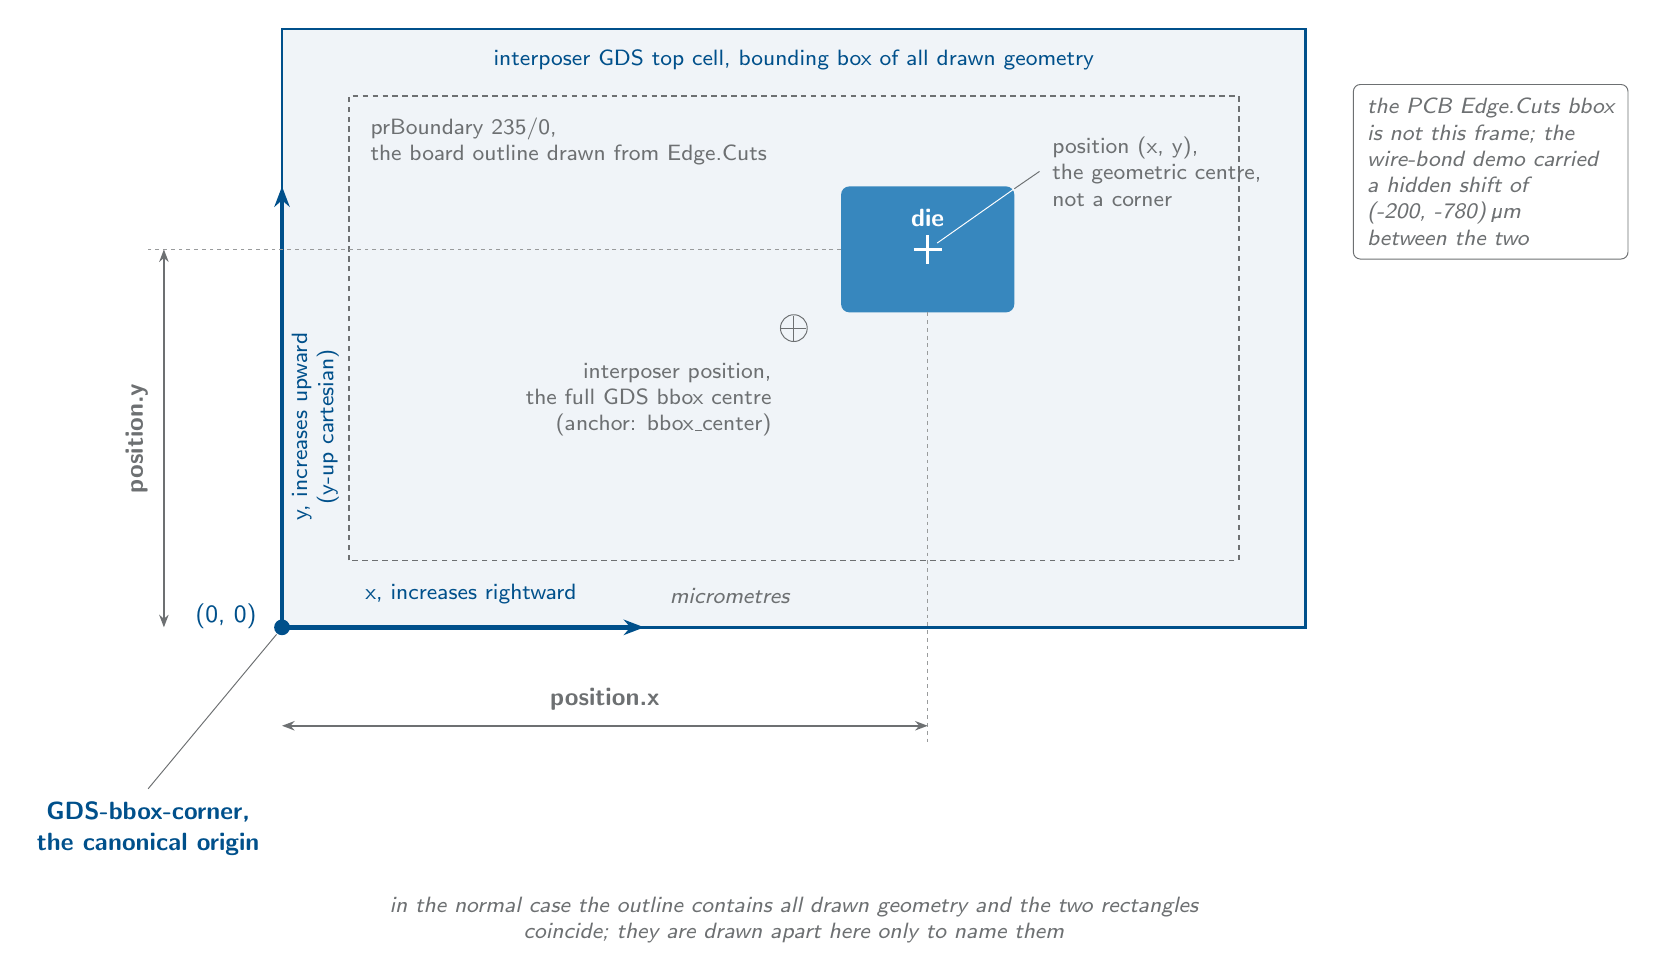
\begin{tikzpicture}[
    >=Stealth,
    adkouter/.style={
        draw=IHPfg, line width=0.9pt, fill=IHPfg!6
    },
    adkinner/.style={
        draw=IHPaccent, line width=0.6pt, dash pattern=on 2pt off 1.6pt
    },
    adkaxis/.style={
        draw=IHPfg, line width=1.6pt, -{Stealth[length=2.6mm]}
    },
    adkdim/.style={
        draw=IHPaccent, line width=0.6pt,
        {Stealth[length=1.6mm]}-{Stealth[length=1.6mm]}
    },
    adkdrop/.style={
        draw=IHPaccent!70, line width=0.35pt, dash pattern=on 1.4pt off 1.4pt
    },
    adkleader/.style={
        draw=IHPaccent, line width=0.35pt
    },
    adklbl/.style={
        font=\sffamily\footnotesize, text=IHPfg, align=center
    },
    adkgrey/.style={
        font=\sffamily\footnotesize, text=IHPaccent, align=center
    },
    adknote/.style={
        font=\sffamily\footnotesize\itshape, text=IHPaccent, align=center
    },
    adkdimlbl/.style={
        font=\sffamily\small\bfseries, text=IHPaccent
    },
    adkcallout/.style={
        font=\sffamily\small\bfseries, text=IHPfg, align=center
    },
    adkdielbl/.style={
        font=\sffamily\small\bfseries, text=white
    }
]

% ---------------------------------------------------------------- reference
% Outer rectangle: the full GDS bounding box of the interposer top cell.
\draw[adkouter] (0,0) rectangle (13.0,7.6);
\node[adklbl, anchor=north] at (6.5,7.45)
    {interposer GDS top cell, bounding box of all drawn geometry};

% Inner rectangle: the board outline drawn from Edge.Cuts.
\draw[adkinner] (0.85,0.85) rectangle (12.15,6.75);
\node[adkgrey, anchor=north west, align=left] at (1.0,6.6)
    {prBoundary 235/0,\\the board outline drawn from Edge.Cuts};

% ---------------------------------------------------------------- axes
\draw[adkaxis] (0,0) -- (4.6,0);
\draw[adkaxis] (0,0) -- (0,5.6);
\node[adklbl, anchor=south] at (2.4,0.18) {x, increases rightward};
\node[adknote, anchor=south west] at (4.80,0.18) {micrometres};
\node[adklbl, rotate=90, anchor=north, align=center, inner sep=1pt]
    at (0.08,2.55)
    {y, increases upward\\(y-up cartesian)};

% ---------------------------------------------------------------- die
\fill[cDieA, rounded corners=3pt] (7.1,4.0) rectangle (9.3,5.6);
\node[adkdielbl] at (8.2,5.20) {die};
% geometric centre marker
\draw[white, line width=1.0pt] (8.02,4.80) -- (8.38,4.80);
\draw[white, line width=1.0pt] (8.20,4.62) -- (8.20,4.98);

% leader out of the die to the position label
\draw[white, line width=0.35pt] (8.32,4.88) -- (9.30,5.57);
\draw[adkleader] (9.30,5.57) -- (9.62,5.79);
\node[adkgrey, anchor=west, align=left] at (9.66,5.79)
    {position (x, y),\\the geometric centre,\\not a corner};

% ---------------------------------------------------------------- interposer position
\draw[adkleader] (6.34,3.80) -- (6.66,3.80);
\draw[adkleader] (6.50,3.64) -- (6.50,3.96);
\draw[adkleader] (6.50,3.80) circle (0.17);
\node[adkgrey, anchor=north east, align=right] at (6.34,3.48)
    {interposer position,\\the full GDS bbox centre\\(anchor: bbox\_center)};

% ---------------------------------------------------------------- origin
\fill[IHPfg] (0,0) circle (0.10);
\node[font=\sffamily\small, text=IHPfg, anchor=east] at (-0.20,0.14) {(0, 0)};
\draw[adkleader] (-1.70,-2.05) -- (-0.07,-0.09);
\node[adkcallout, anchor=north] at (-1.70,-2.10)
    {GDS-bbox-corner,\\the canonical origin};

% ---------------------------------------------------------------- measurements
% witness lines from the die centre
\draw[adkdrop] (7.10,4.80) -- (-1.72,4.80);
\draw[adkdrop] (8.20,4.00) -- (8.20,-1.48);

\draw[adkdim] (0,-1.25) -- (8.20,-1.25);
\node[adkdimlbl, anchor=south] at (4.10,-1.18) {position.x};

\draw[adkdim] (-1.50,0) -- (-1.50,4.80);
\node[adkdimlbl, rotate=90, anchor=south] at (-1.58,2.40) {position.y};

% ---------------------------------------------------------------- side note
\node[anchor=north west, align=left,
      font=\sffamily\footnotesize\itshape, text=IHPaccent,
      draw=IHPaccent, line width=0.35pt, rounded corners=2.5pt,
      inner sep=5pt]
    at (13.60,6.90)
    {the PCB Edge.Cuts bbox\\
     is not this frame; the\\
     wire-bond demo carried\\
     a hidden shift of\\
     (-200, -780)\,\textmu m\\
     between the two};

% ---------------------------------------------------------------- footnote
\node[adknote, anchor=north] at (6.50,-3.30)
    {in the normal case the outline contains all drawn geometry and the two
     rectangles\\coincide; they are drawn apart here only to name them};

\end{tikzpicture}
\end{document}
